\documentclass[a4paper, 10pt]{report}
\usepackage[italian]{babel}
\usepackage[T1]{fontenc}
\usepackage[utf8]{inputenc}
\usepackage{charter}
\usepackage{amsmath}
\usepackage{amsthm}
\usepackage{amsfonts}
\usepackage{graphicx}
\usepackage{wrapfig}
\usepackage{tcolorbox}
\usepackage{fancyhdr}
\usepackage{listings}
\usepackage{longtable}
\usepackage{multicol}
\usepackage{xcolor}

\usepackage{geometry}
\geometry{a4paper, left=2cm,right=2cm,top=2cm,bottom=2cm}

\pagestyle{fancy}
\lhead{}
\chead{}
\rhead{\bfseries 17 ottobre 2019 }
\lhead{\bfseries Segnali e immagini - laboratorio}

\newcounter{main}
\setcounter{main}{1}

\lstnewenvironment{code}[1][firstnumber=\themain,name=main]
  {\lstset{language=matlab,
           basicstyle=\medium\ttfamily,
           numbers=left,
           basicstyle=\small,
           columns=fullflexible,
           #1
          }
}
{\setcounter{main}{\value{lstnumber}}}


\begin{document}

\section*{\underline{Cross - correlazione con matlab}}

\textbf{Esempio di cross - correlazione:}

\begin{code}
f1 = [1 1 1 1 1 1 1 1]; %box 
f2 = [1 2 3 4 5 6 7 8]; %triangolo

figure; set(gcf,'name','Cross Correlazione','IntegerHandle','off');
subplot(311); stem(f1);
subplot(312); stem(f2);
[f1xf2,lag] = xcorr(f1,f2);
subplot(313); plot(lag,f1xf2); hold; stem(lag,f1xf2);
\end{code}

\noindent \\Analisi codice:

\begin{longtable}{| p{.15\textwidth} | p{.80\textwidth} |}

\textbf{figure} & Crea una nuova sottofinestra.
\\
\hrule & \hrule
\\
\textbf{subplot(nmp)} & Suddivide la sottofinestra in una matrice di n righe e m colonne. Il valore p indica la posizione della "cella" in cui operare.
\\
\hrule & \hrule
\\
\textbf{stem(array)} & Basandosi su array, crea sul grafico dei segmenti terminati con un pallino (serve per disegnare segnali discreti).
\\
\textbf{stem(x, y)} & Crea un segmento in posizione x alto y, terminante con un pallino.
\\
\hrule & \hrule
\\
\textbf{xcorr(s1, s2)} & Esegue la cross - correlazione tra s1 e s2. Ritorna due array differenti: il prima riporta il valore della cross correlazione per ogni punto di shift, mentre il secondo riporta lo shift del segnale s2. 
\\
\hrule & \hrule
\\
\textbf{plot(x, y)} & Crea un grafico (continuo) a partire dagli array x e y.
\\
\end{longtable}

\noindent Risultato:

\begin{center}
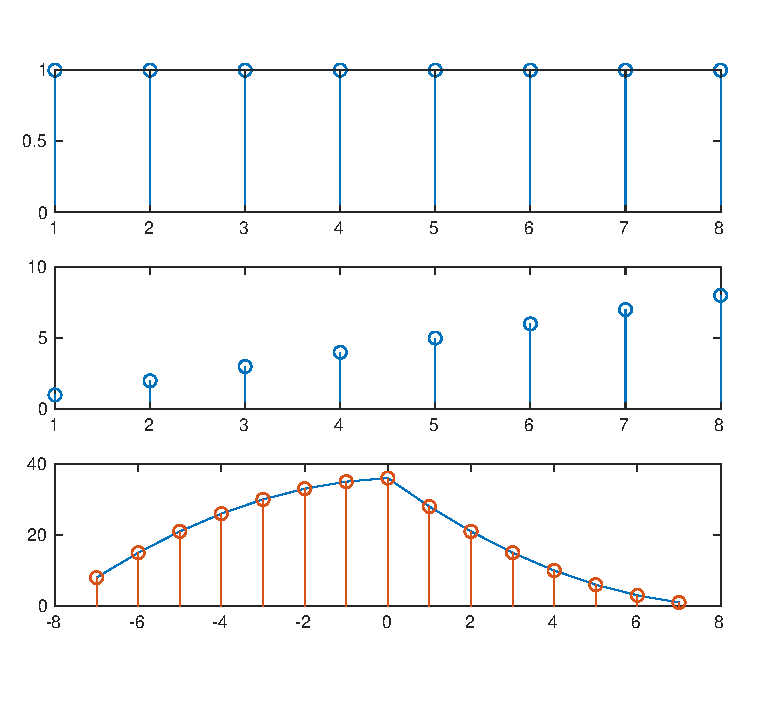
\includegraphics[scale=1]{es1.pdf}
\end{center}

\end{document}